\chapter{Resultados}
    Con el fin de demostrar la correcta funcionalidad de los módulos descritos en el capitulo 4, en el presente apartado se exponen los diversos resultados obtenidos a lo largo del desarrollo del prototipo. Por discreción, los datos sensibles fueron enmascarados.
    
    \section{Módulo de extracción (\textit{Scraper})}
    Este módulo basa su funcionalidad en la conectividad exitosa con \textit{Graph API} de Facebook para poder dar lugar a la descarga de conversaciones que serán empleadas por el agente conversacional después de haber sido normalizadas. Como se menciono en la sección 4, al descargar las conversaciones se busca que exista una base de datos no relacional disponible, de ser así entonces las conversaciones serán almacenadas en dicha base de datos (figura \ref{fig:almacenamiento-db-nosql}), en caso contrario en el sistema local de archivos (figura \ref{fig:almacenamiento-local-conversacion}, \ref{fig:almacenamiento-local-mensaje} y \ref{fig:almacenamiento-local-mensaje-editor}).
    
    \begin{figure}[H]
         \centering
         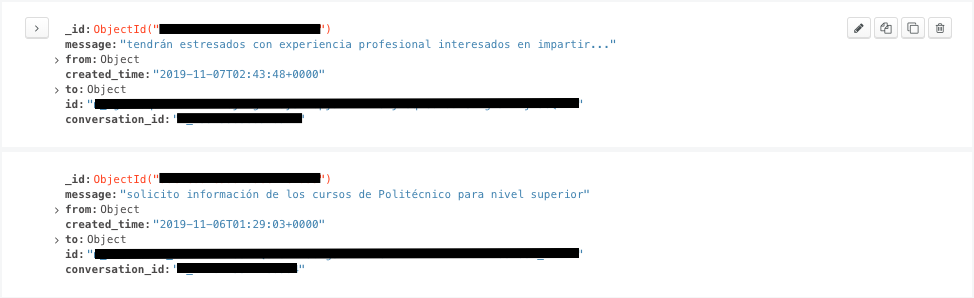
\includegraphics[height=7cm, width=16.5cm]{Latex/Classes/Imagenes/almacenamiento-db-nosql.png}
         \caption{Datos crudos obtenidos de \textit{Graph API} almacenados en base de datos \textit{NoSQL}.}
         \label{fig:almacenamiento-db-nosql}
    \end{figure}
    
    \begin{multicols}{2}
        \begin{figure}[H]
             \centering
             
\includegraphics[height=2.5cm, width=6cm]{Latex/Classes/Imagenes/almacenamiento-local.png}
             \caption{Datos crudos obtenidos de \textit{Graph API} almacenados en el sistema local de archivos por conversación.}
             \label{fig:almacenamiento-local-conversacion}
        \end{figure}
        
        \begin{figure}[H]
             \centering
             
\includegraphics[height=2.5cm, width=6cm]{Latex/Classes/Imagenes/conversacion-local.png}
             \caption{Datos crudos obtenidos de \textit{Graph API} almacenados en el sistema local de archivos por mensaje.}
             \label{fig:almacenamiento-local-mensaje}
        \end{figure}
    \end{multicols}
    \begin{figure}[H]
         \centering
         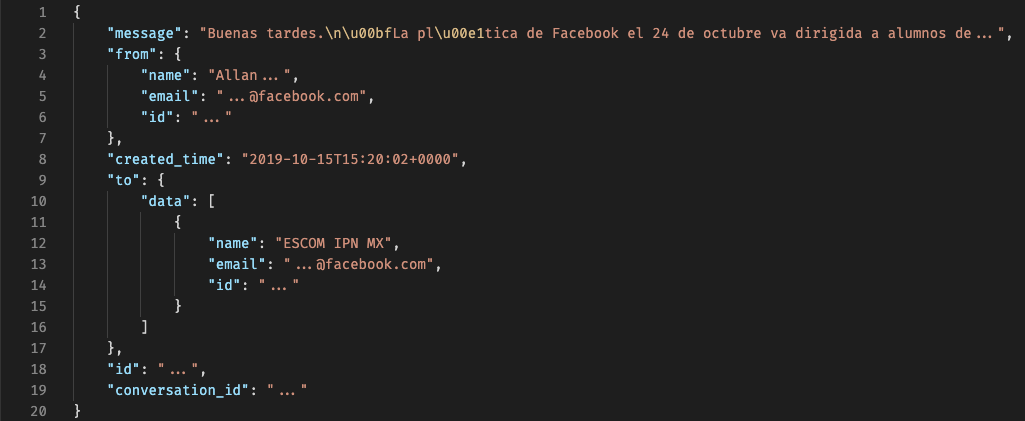
\includegraphics[height=6cm, width=16.5cm]{Latex/Classes/Imagenes/conversacion-local-vista.png}
         \caption{Datos crudos obtenidos de \textit{Graph API} almacenados en el sistema local de archivos visto desde un editor de texto.}
         \label{fig:almacenamiento-local-mensaje-editor}
    \end{figure}
    
    \section{Módulo de procesamiento de lenguaje natural}
    Una vez que se tiene una base de datos \textit{NoSQL} disponible y además, alimentada con los datos crudos gracias a \textit{Graph API}, el módulo de procesamiento de lenguaje natural hace disposición de estos datos para limpiarlos y almacenarlos en una base de datos relacional (véase la figura \ref{fig:diagrama-entidad-relacion}) en cada una de sus etapas de normalización como se puede ver en la figura \ref{fig:sql-message-table}, es decir:
    \begin{itemize}
        \item Mensaje crudo: Mensaje tal cual es extraído de \textit{Graph API}.
        \item Mensaje con stopwords y sin lemas: Mensaje sin cualquier carácter que no pertenezca al abecedario latino.
        \item Mensaje sin stopwords y sin lemas: Mensaje sin cualquier carácter que no pertenezca al abecedario latino y sin \textit{stopwords}.
        \item Mensaje sin stopwords y con lemas: Mensaje sin cualquier carácter que no pertenezca al abecedario latino, sin \textit{stopwords} y lematizado. 
        \item Mensaje con stopwords y con lemas: Mensaje sin cualquier carácter que no pertenezca al abecedario latino y lematizado. 
    \end{itemize}
    
    \begin{figure}[H]
         \centering
         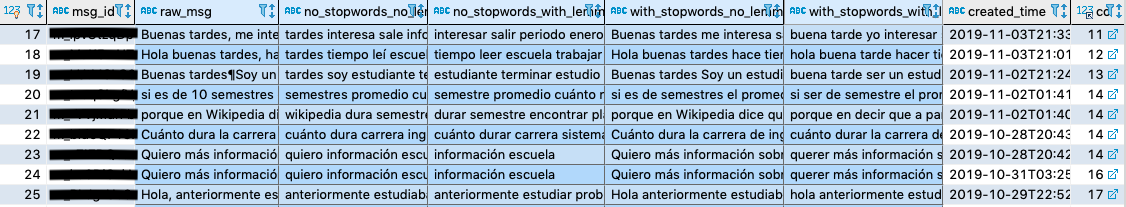
\includegraphics[height=4cm, width=16.5cm]{Latex/Classes/Imagenes/message-table.png}
         \caption{Datos en diferentes niveles de normalización almacenados en la base de datos relacional.}
         \label{fig:sql-message-table}
    \end{figure}

    \begin{figure}[H]
         \centering
         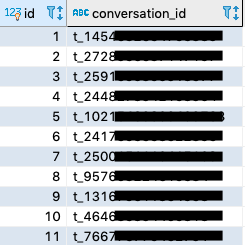
\includegraphics[height=6cm, width=8cm]{Latex/Classes/Imagenes/conversation-table.png}
         \caption{Tabla de conversaciones.}
         \label{fig:sql-conversation-table}
    \end{figure}
    
    Una vez realizada la normalización, se extraen los datos de cada una de las columnas descritas anteriormente para poder realizar un análisis de tópicos, a continuación se muestran los resultados. \newpage
    
    \begin{itemize}
        \item De los mensajes con \textit{stopwords} y sin lemas no se pudo obtener gran información puesto que las palabras que predominan son palabras vacías como artículos, pronombres, preposiciones, etc.
        \begin{figure}[H]
            \centering
            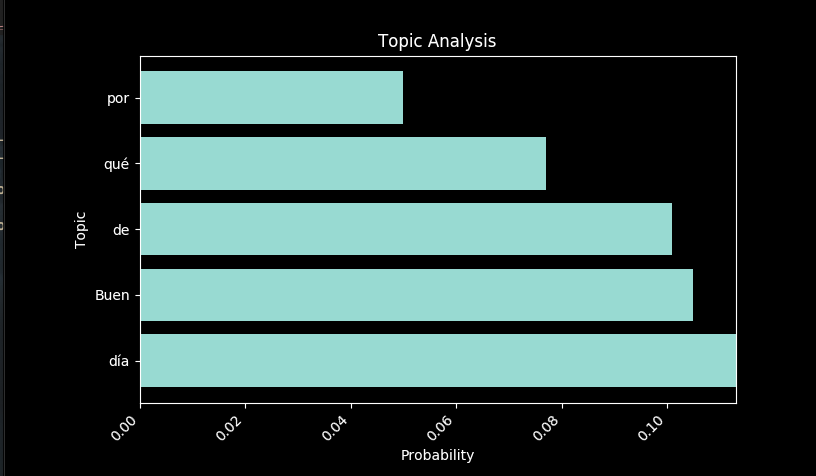
\includegraphics[height=8cm, width=16.5cm]{Latex/Classes/Imagenes/ws_nl-1.png}
            \caption{Resultado \textbf{LDA} con documentos con \textit{stopwords} y sin lemas (a).}
            \label{fig:ws_nl-1}
        \end{figure}
        \begin{figure}[H]
            \centering
            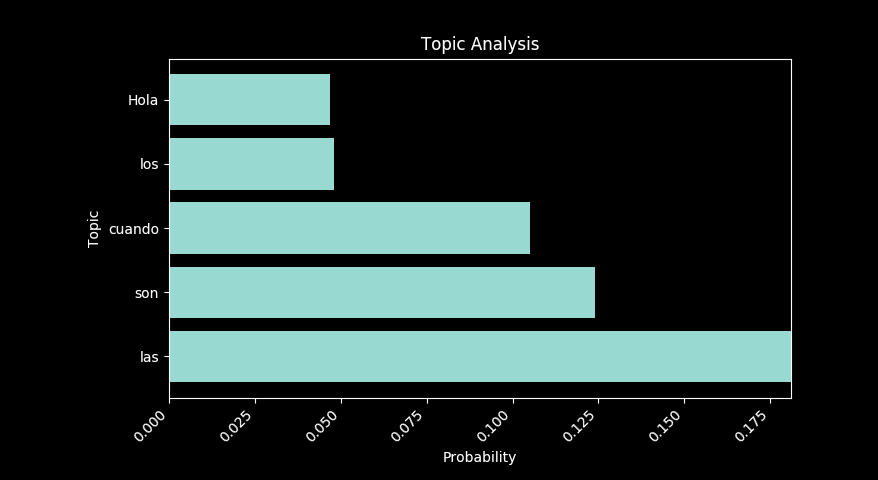
\includegraphics[height=8cm, width=16.5cm]{Latex/Classes/Imagenes/ws_nl-2.png}
            \caption{Resultado \textbf{LDA} con documentos con \textit{stopwords} y sin lemas (b).}
            \label{fig:ws_nl-2}
        \end{figure}
        \newpage
        
        \item De los mensajes con \textit{stopwords} y con lemas no se pudo obtener gran información puesto que las palabras que predominan siguen siendo palabras vacías como artículos, pronombres, preposiciones, etc., a pesar de que el texto se encuentre lematizado.
        \begin{figure}[H]
            \centering
            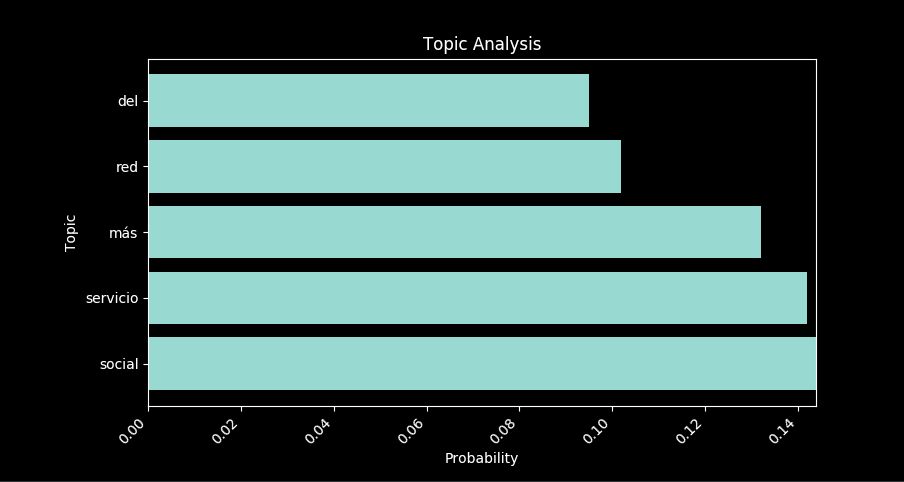
\includegraphics[height=8cm, width=16.5cm]{Latex/Classes/Imagenes/ws_wl-1.png}
            \caption{Resultado \textbf{LDA} con documentos con \textit{stopwords} y con lemas (a).}
            \label{fig:ws_wl-1}
        \end{figure}
        \begin{figure}[H]
            \centering
            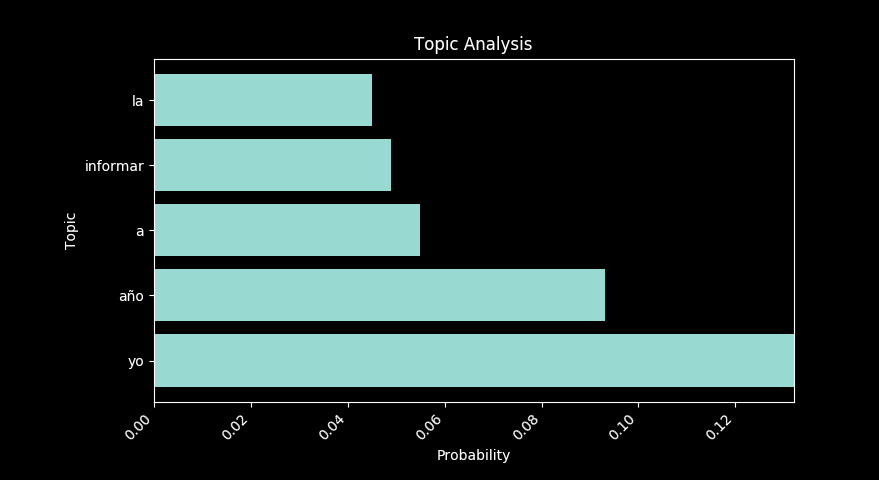
\includegraphics[height=8cm, width=16.5cm]{Latex/Classes/Imagenes/ws_wl-2.png}
            \caption{Resultado \textbf{LDA} con documentos con \textit{stopwords} y con lemas (b).}
            \label{fig:ws_wl-2}
        \end{figure}
        \newpage
        
        \item De los mensajes sin \textit{stopwords} y sin lemas los resultados obtenidos dieron lugar un avance significativo en los resultados, puesto que se pudieron encontrar temas relevantes de interés entre los estudiantes como: tramite de baja temporal, convocatorias de exámenes de admisión, inscripciones, información sobre el plantel e incluso ofertas laborales.
        \begin{figure}[H]
            \centering
            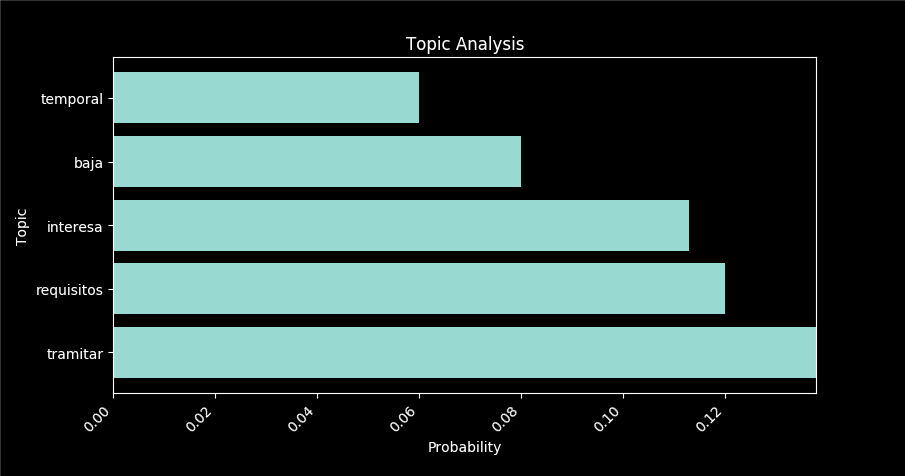
\includegraphics[height=8cm, width=16.5cm]{Latex/Classes/Imagenes/ns_nl-1.png}
            \caption{Resultado \textbf{LDA} con documentos sin \textit{stopwords} y sin lemas (a).}
            \label{fig:ns_nl-1}
        \end{figure}
        \begin{figure}[H]
            \centering
            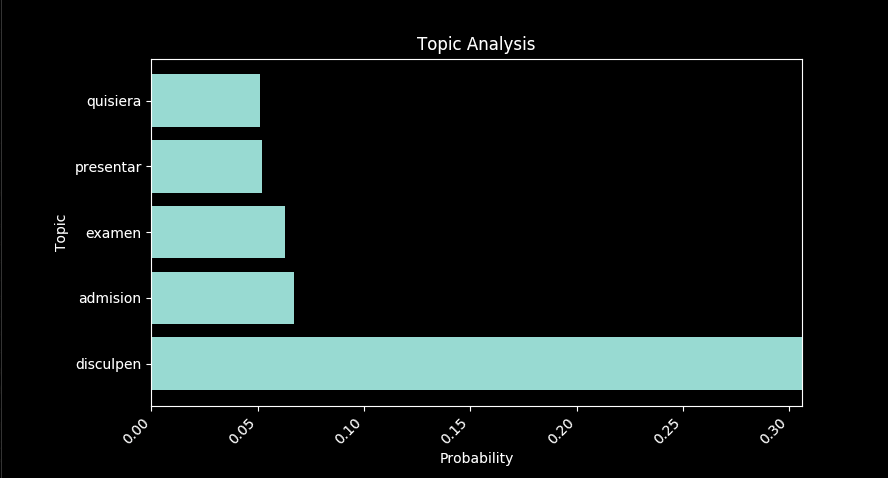
\includegraphics[height=8cm, width=16.5cm]{Latex/Classes/Imagenes/ns_nl-2.png}
            \caption{Resultado \textbf{LDA} con documentos sin \textit{stopwords} y sin lemas (b).}
            \label{fig:ns_nl-2}
        \end{figure}
        \begin{figure}[H]
            \centering
            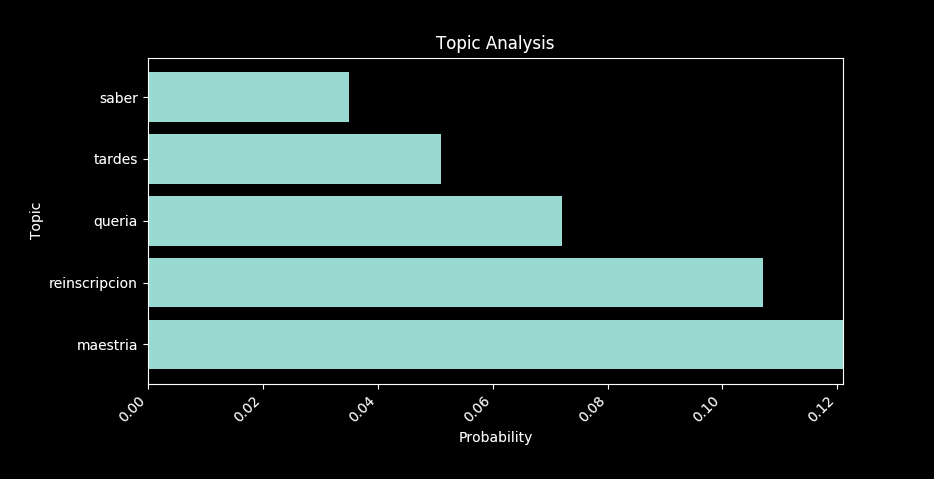
\includegraphics[height=8cm, width=16.5cm]{Latex/Classes/Imagenes/ns_nl-3.png}
            \caption{Resultado \textbf{LDA} con documentos sin \textit{stopwords} y sin lemas (c).}
            \label{fig:ns_nl-3}
        \end{figure}
        \begin{figure}[H]
            \centering
            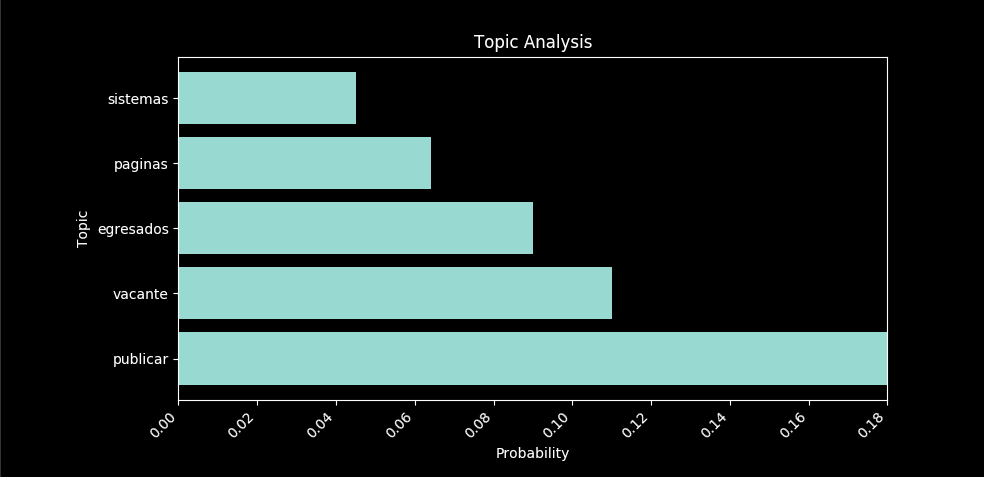
\includegraphics[height=8cm, width=16.5cm]{Latex/Classes/Imagenes/ns_nl-4.png}
            \caption{Resultado \textbf{LDA} con documentos sin \textit{stopwords} y sin lemas (d).}
            \label{fig:ns_nl-4}
        \end{figure}
        \begin{figure}[H]
            \centering
            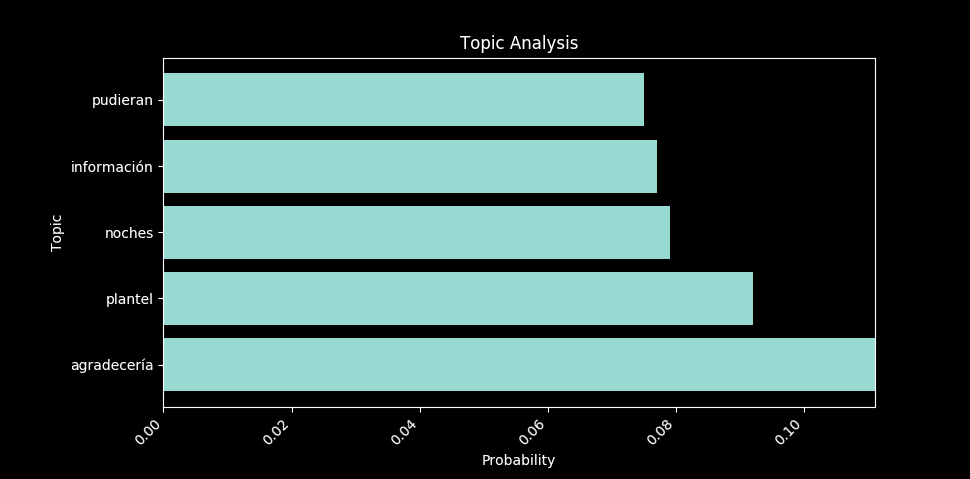
\includegraphics[height=8cm, width=16.5cm]{Latex/Classes/Imagenes/ns_nl-5.png}
            \caption{Resultado \textbf{LDA} con documentos sin \textit{stopwords} y sin lemas (e).}
            \label{fig:ns_nl-5}
        \end{figure}
        \begin{figure}[H]
            \centering
            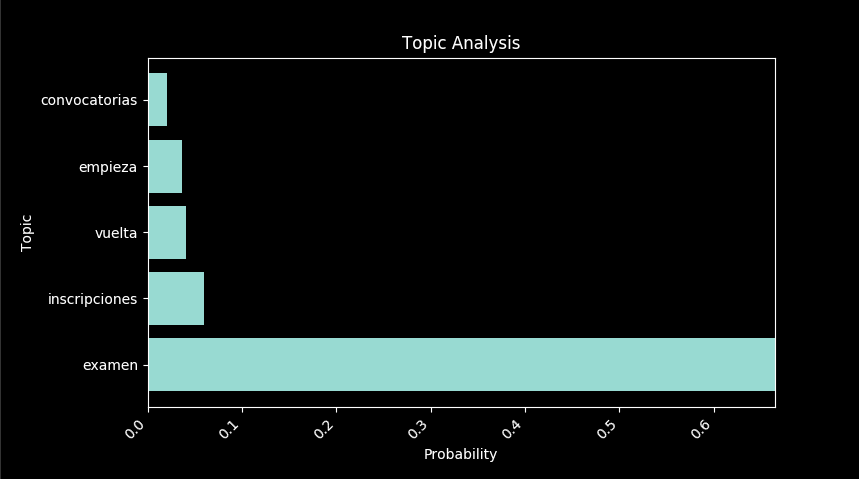
\includegraphics[height=8cm, width=16.5cm]{Latex/Classes/Imagenes/ns_nl-6.png}
            \caption{Resultado \textbf{LDA} con documentos sin \textit{stopwords} y sin lemas (f).}
            \label{fig:ns_nl-6}
        \end{figure}
        \newpage
        
        \item De los mensajes sin \textit{stopwords} y con lemas, probablemente dieron lugar a los resultados esperados ya que la mayoría de los estudiantes están interesados en los siguientes tópicos: exámenes de ingreso, cambio de carrera, convocatoria de titulación, convocatoria para inscripción a maestría, bajas temporales, taller de protocolo de trabajo terminal, servicio social, etc.
        \begin{figure}[H]
            \centering
            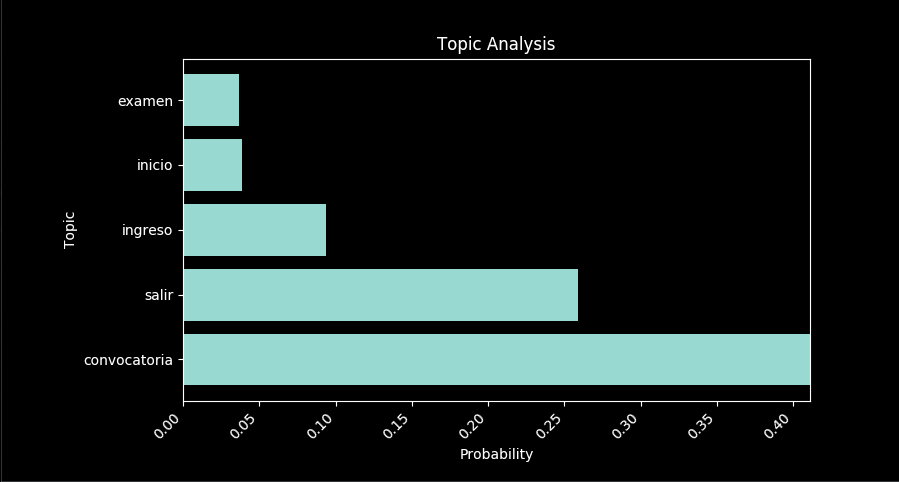
\includegraphics[height=8cm, width=16.5cm]{Latex/Classes/Imagenes/ns_wl-1.png}
            \caption{Resultado \textbf{LDA} con documentos sin \textit{stopwords} y con lemas (a).}
            \label{fig:ns_wl-1}
        \end{figure}
        \begin{figure}[H]
            \centering
            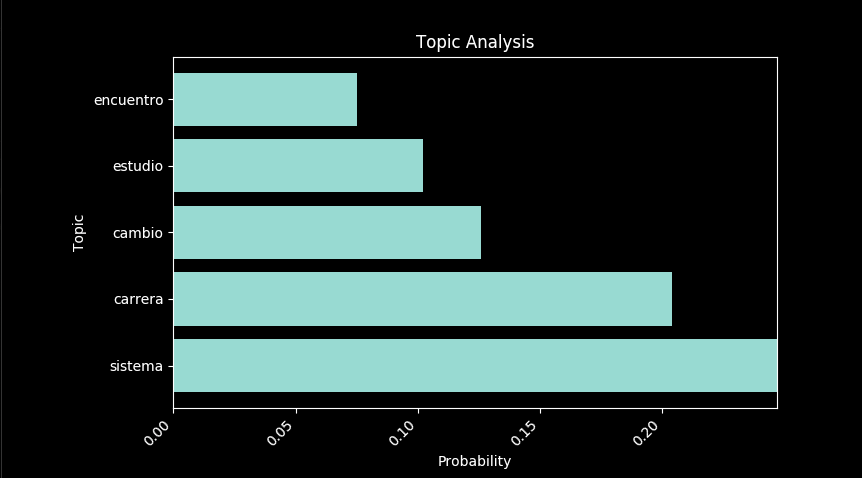
\includegraphics[height=8cm, width=16.5cm]{Latex/Classes/Imagenes/ns_wl-2.png}
            \caption{Resultado \textbf{LDA} con documentos sin \textit{stopwords} y con lemas (b).}
            \label{fig:ns_wl-2}
        \end{figure}
        \begin{figure}[H]
            \centering
            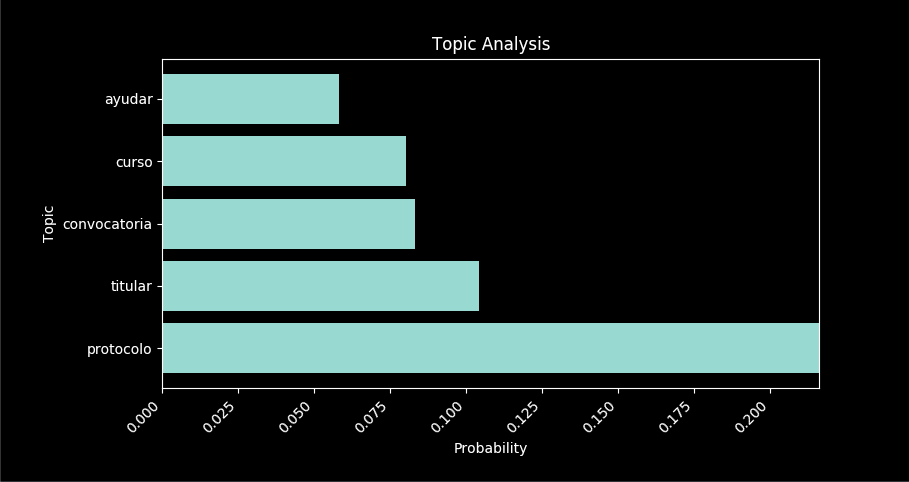
\includegraphics[height=8cm, width=16.5cm]{Latex/Classes/Imagenes/ns_wl-3.png}
            \caption{Resultado \textbf{LDA} con documentos sin \textit{stopwords} y con lemas (c).}
            \label{fig:ns_wl-3}
        \end{figure}
        \begin{figure}[H]
            \centering
            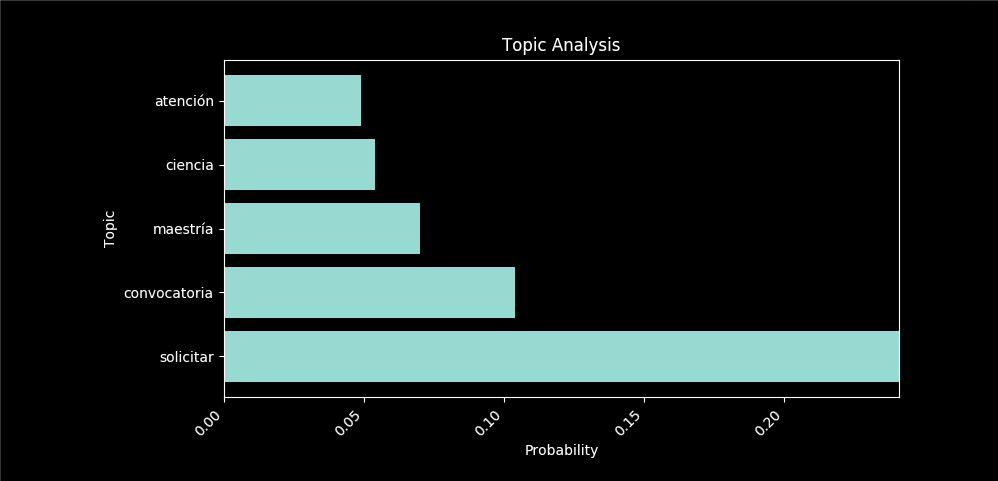
\includegraphics[height=8cm, width=16.5cm]{Latex/Classes/Imagenes/ns_wl-4.png}
            \caption{Resultado \textbf{LDA} con documentos sin \textit{stopwords} y con lemas (d).}
            \label{fig:ns_wl-4}
        \end{figure}
        \begin{figure}[H]
            \centering
            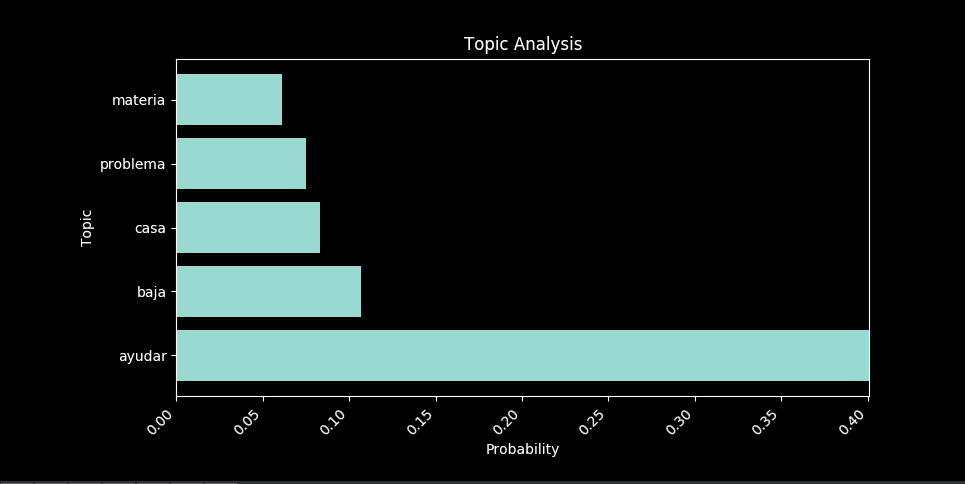
\includegraphics[height=8cm, width=16.5cm]{Latex/Classes/Imagenes/ns_wl-5.png}
            \caption{Resultado \textbf{LDA} con documentos sin \textit{stopwords} y con lemas (e).}
            \label{fig:ns_wl-5}
        \end{figure}
        \begin{figure}[H]
            \centering
            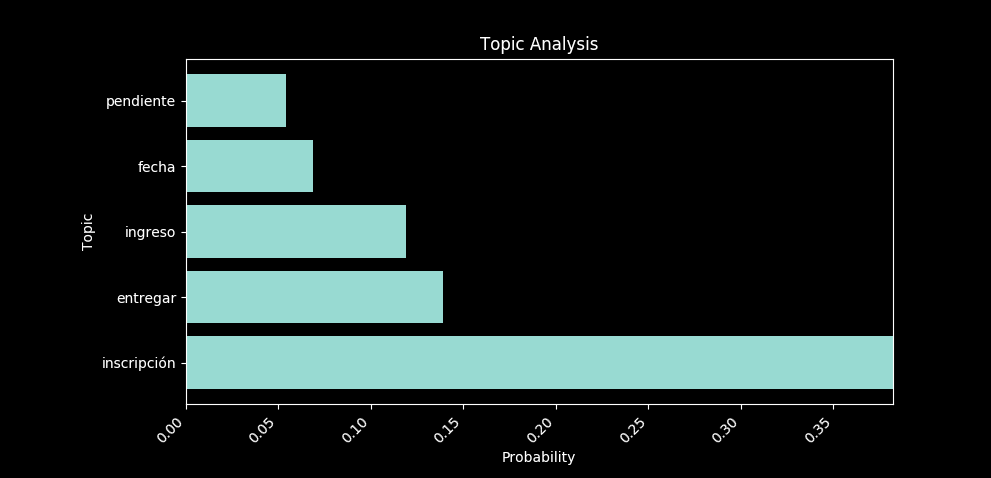
\includegraphics[height=8cm, width=16.5cm]{Latex/Classes/Imagenes/ns_wl-6.png}
            \caption{Resultado \textbf{LDA} con documentos sin \textit{stopwords} y con lemas (f).}
            \label{fig:ns_wl-6}
        \end{figure}
        \begin{figure}[H]
            \centering
            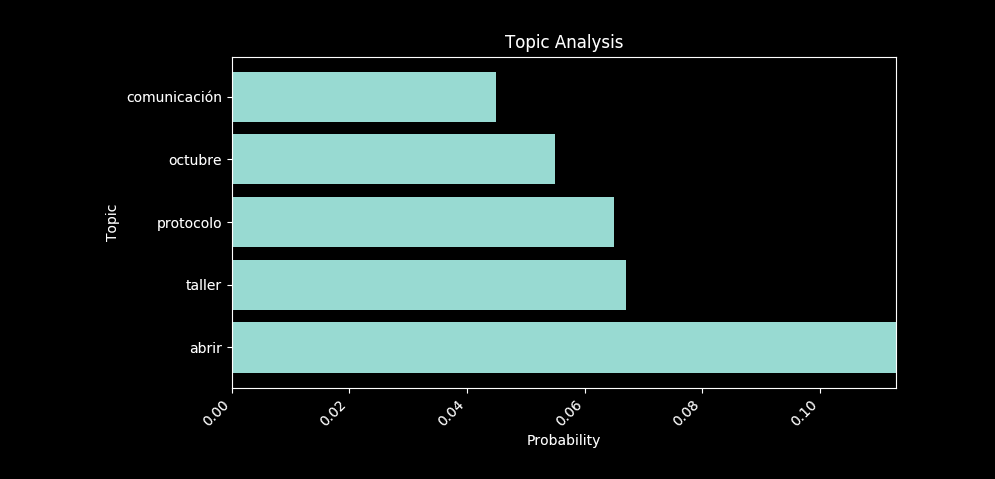
\includegraphics[height=8cm, width=16.5cm]{Latex/Classes/Imagenes/ns_wl-7.png}
            \caption{Resultado \textbf{LDA} con documentos sin \textit{stopwords} y con lemas (g).}
            \label{fig:ns_wl-7}
        \end{figure}
        \begin{figure}[H]
            \centering
            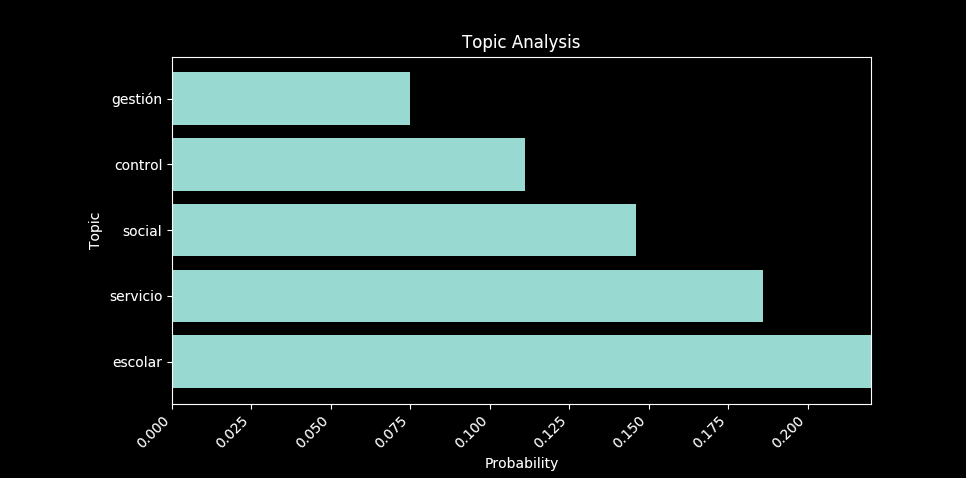
\includegraphics[height=8cm, width=16.5cm]{Latex/Classes/Imagenes/ns_wl-8.png}
            \caption{Resultado \textbf{LDA} con documentos sin \textit{stopwords} y con lemas (h).}
            \label{fig:ns_wl-8}
        \end{figure}
        
    \end{itemize}